% \subsection{Colour rendering and light quality specification}

% Colour rendering indices provide an indication of the colour appearance of objects under a test illumination. Colour fidelity indices (properly a subset of colour rendering indices, however the most commonly used colour rendering index is in fact a colour fidelity index) are designed to describe how well a light source will produce a faithful appearance in terms of corresponding colorimetry to an appearance under \gls{CIE} D-series illuminant (daylight proxy) or a black body radiator. Target values are generally provided in museum lighting guidelines \citep{ies_ies_1996,druzik_guidelines_2012,cibse_lighting_2015,thomson_museum_1986}. The recommended value for the ubiquitously used \gls{CIE} R\textsubscript{a} (As defined in \gls{CIE} 13.3:1995 \citep{cie_cie_1995}), often informally referred to as `CRI', varies from publication to publication, but is generally \gls{CIE} R\textsubscript{a}$>$80, but with no experimental work referenced to support this figure. Research in colour rendering is at a point of change and development, with the recognition that a single figure might never be enough to describe the complex, multidimensional, subjective and context dependent qualia of colour rendering\citep{rea_color_2008}. Thus new indices, and modifications and addenda to long-established indices are being proposed \citep{smet_memory_2012,davis_color_2010,rea_practical_2010,color_metric_task_group_of_the_ies_ies_2015,teunissen_characterising_2016}.

% To discuss the colour rendering of a light source is to discuss the colour appearance of objects which the light source's illumination may facilitate. 

% If we were to take a bunch of balloons (or any objects, but balloons provide a simple and vivid image in the minds of most) of varied and multiple colours, from an area lit with daylight to an area lit with artificial light, and the colour appearance changes, for example the colours become more dull, we would generally be disappointed, understandably so. In this case, we could say that we were dissatisfied by the colour rendering qualities of the artificial light source. If the colours remained the same we probably would think little of it, but if we were pressed for a comment, we might say that the colour appearance was satisfactory.

% If the balloons stayed the same colour what we'd be seeing specifically is a high level of colour fidelity, fidelity meaning faithfulness or truthfulness. If fidelity aligns well with the priorities of the user, then high levels of fidelity are desirable. It is assumed when discussing colour fidelity generally, that we're actually discussing fidelity to appearance under daylight or sometimes a Planckian radiator, aka a black body radiator. This is a fine comparison, but one which should be consciously considered; fidelity is not a measure of a light source per se, it is a comparison of that light source to a reference illuminant.

% Fidelity has long been considered semi-analogous for colour rendering as a whole, but it should be remembered that it is really only one element of colour rendering, albeit one with useful correlation to others. Here I should point out that the \gls{CIE} definition of colour rendering, from the publication \gls{CIE} S 017/E:2011 ILV: International Lighting Vocabulary \citep{cie_cie_2011} reads: ``Effect of an illuminant on the colour appearance of objects by conscious or subconscious comparison with their colour appearance under a reference illuminant.'' You'll notice the similarities to the definition I have ascribed to colour fidelity, and specifically not colour rendering. This is an unfortunate clash of nomenclature which I see as inappropriate usage on the part of \gls{CIE}, and at some point I hope this official definition will be updated to match the modern vernacular.

% When considering how `good' a light source is at facilitating colour with the objects which it illuminates, we might consider different measures alongside or in place of fidelity.

% \begin{itemize}
% \item \emph{Colour Fidelity (to recap)} - A measure of comparison between how colours appear under daylight (or other reference) and how they appear under another light source. %Do the balloons appear the same colour indoors and out? Are individual colours important or is an average suitably representative?
% \item \emph{Chromatic Discrimination} - The ability of a light source to illuminate objects such that subtle differences in colour are made most visible. %Can you tell the difference between all the balloons? How big are the differences? Are threshold differences more or less important than the perceived magnitude of suprathreshold differences?
% \item \emph{Observer Preference} - Subjective preferences for the colour of objects, potentially related to an increase in saturation, or an observer's memory of colours, or specific colour effects (e.g. enhanced skin tones). %Do the balloons look `nicer'/more vivid/more like the last time you saw them?
% \end{itemize}

% These areas overlap, and often exhibit correlation. For example, if a light source has properties which allow for high fidelity rendering, quite often that light source might also allow for good colour discrimination and also facilitate colours which might appear natural and/or pleasing. These are not reliable correlations however; it is quite possible to have a light source with very dissimilar properties to daylight that could score highly on discrimination and/or preference, or vice versa.

% The index in widest use currently for quantifying colour rendering is \gls{CIE} R\textsubscript{a} (The General Colour Rendering Index). At start of my studies, this metric almost exclusively to generate the figure listed as `CRI' or similar on the packaging for bulbs available commercially. %In the intervening time, IES RP-30-15\cite{color_metric_task_group_of_the_ies_ies_2015}, and more recently IES RP-30-18\cite{ies_ies_2018}, have been published. %and...

% \gls{CIE} R\textsubscript{a} is a colour fidelity metric, produced by computing the colour differences of 8 specified test colour samples (TCSs), between the situation where illumination is provided by the test source and that where it is provided by a reference illuminant with the same \gls{CCT} as the test source, and taking the arithmetic mean of these colour differences. The index is scaled such that the highest score is 100, for light sources which reproduce the TCSs under the reference illuminant exactly, with any light source which induces a colour shift receiving a value less than 100, descending below 0 if the magnitude of the shifts are great enough.

% The most recent version of the standard specifying this metric is `\gls{CIE} 13.3-1995 Method of Measuring and Specifying Colour Rendering Properties of Light Sources' \citep{cie_cie_1995}. This document briefly overviews the history of, and necessity for, a colour rendering index and highlights areas of the procedure which vary compared to previous recommendations, and clearly details the recommended procedure. The process is summarised in the flow chart of Figure \ref{fig:criflow}. For a worked example see \citet[p.388]{hunt_measuring_2011}.

% In response to a lack of confidence that \gls{CIE} R\textsubscript{a} delivered meaningful values for LED illumination, a considerable amount of research and discussion has revolved around the subject of a colour rendering index to supersede \gls{CIE} R\textsubscript{a}. This is commonly complicated by the assumption that the values obtained from a fidelity index in some way correlate with a visual appearance; \gls{CIE} R\textsubscript{a} does not predict preference between two light sources. A more valid criticism of \gls{CIE} R\textsubscript{a} is that it comprises deprecated methods and data sets for computing intermediary stages within the process of calculation, and thus this theoretically limits the `correctness' of any values produced by it.

% Following many years where multiple \gls{CIE} technical committees aimed to deliver updated colour rendering indices, but subsequently didn't make any firm recommendations, an IES group was formed with the aim of examining the issue. The output of this IES group was the production of IES TM-30-15\cite{color_metric_task_group_of_the_ies_ies_2015}, which follows the same philosophy as \gls{CIE} R\textsubscript{a} but with more modern colour science. It is still a contentious issue whether this updated index genuinely offers advantages over \gls{CIE} R\textsubscript{a}. 
% % it also includes a bunch of other things...
% % and IES TM-30-18?

% Alternative propositions which offer fundamentally different approaches to the evaluation of colour rendering have been offered in recent years, including: 
% \begin{itemize}
% \item indices based on production of memory colours\citep{smet_memory_2012}.
% \item indices which consider the size of the gamut of a TCS set\citep{rea_color_2008,teunissen_characterising_2016}.
% \item indices which are fundamentally fidelity indices but which penalise or reward specific traits known to be disliked/preferred\citep{ohno_rationale_2010}.
% \end{itemize}

% \begin{figure}[htbp]
% 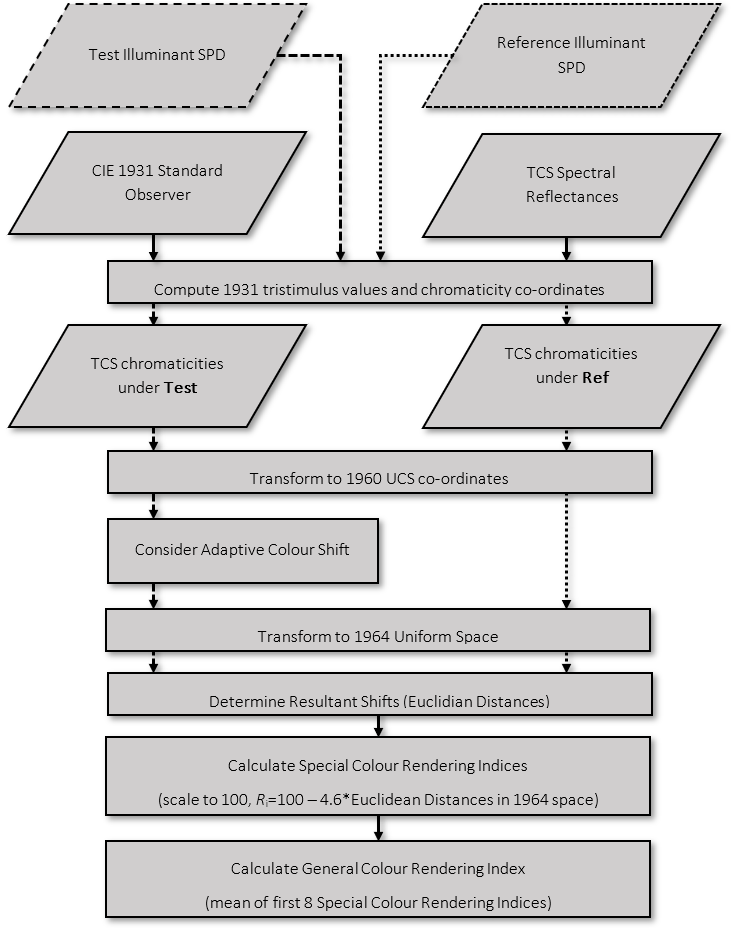
\includegraphics[max width=\textwidth]{figs/LitRev/criflow.png}
% \caption{The stages of calculation for the computation of the \gls{CIE} General Colour Rendering Index. Notes: Reference illuminant: the same or nearly the same \gls{CCT}. Below 5000K reference spectrum will be that of a black body radiator, and from 5000K `one of a series of spectral power distributions of phases of daylight'.}
% \label{fig:criflow}
% \end{figure}

\clearpage